Deep learning is from a mathematical perspective - A method of representing differential functions mapping one type of variable $x$, into another type of variable $y$.

$$
f(In\_variable) = out\_variable
$$

\noindent
In this project, we are gonna focus on two deep learning methods which both are neural networks: Recurrent neural networks(RNNs) and convolutional neural networks(Cnns).

\subsection{neural networks}
A neural network is a type of deep learning model. A neural network is a model that is inspired by how biological neurons work in the brain. A neural network itself has many units called neurons, these neurons are grouped into several layers. These layers are columns of neurons. Each neuron is connected to adjacent layers of neurons through connectors called weights. These weights are functions which are multiplied with the neurons and some bias between layers. These biases are meant to push these functions toward a specific output.

\begin{figure}[!ht]
  \centering
  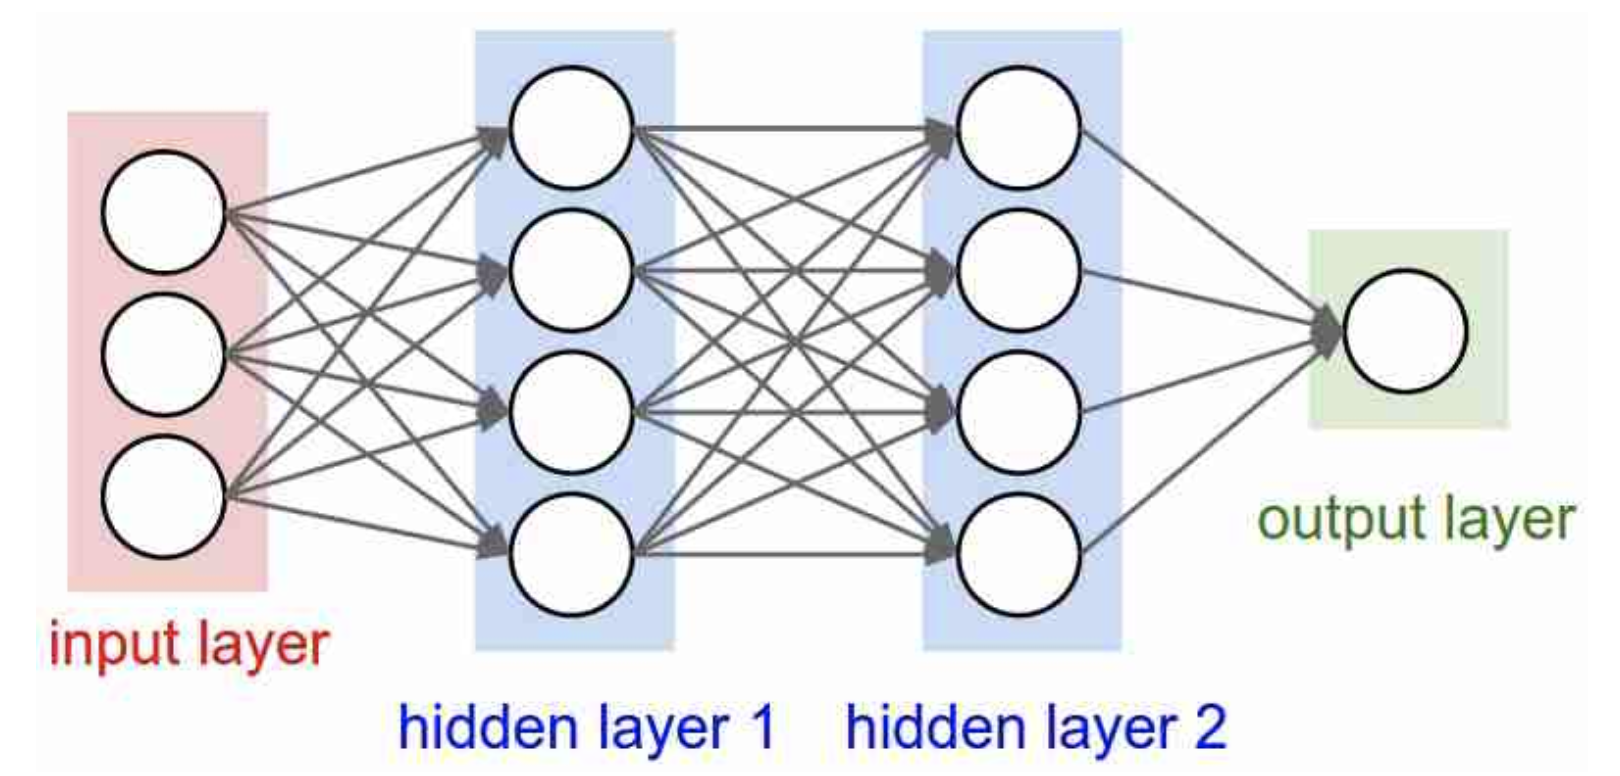
\includegraphics[scale=0.4]{latex/imgs/NN.png}
  \caption{Table}\label{Baseline:before}
\end{figure}

\subsection{RNN - LSTM}
RNNs are strong tools because of the ability of mapping sequences of arbitrary length. A sequence is a set of data, which has a defined order to it. An example of a sequence, could be a sentence in any given language:
\begin{itemize}
    \item I went home from school because of Corona-virus.
\end{itemize}

\noindent
Some of the transformations RNNs can can do, are:
\begin{align*}
	&f:sequence \rightarrow R^D\\
	&f:R^D \rightarrow sequence\\
	&f:sequence \rightarrow sequence
\end{align*}
\noindent
It is because of these general transformations and the way it can be done on sequential data with arbitrary length, that makes RNNs a strong tool. This makes RNNs useful in applications as:
\begin{itemize}
    \item Natural language proccesing(NLP)
    \begin{itemize}
    	\item text generation, autofill, analysis, translation, etc.
    \end{itemize}
    \item Speech, music, and video processing/generation
\end{itemize}

\noindent
RNNs outputs are based on a function of previous steps of outputs. Meaning it takes the previos output and uses it as input. Thus, given the name Recurrent neural network.\\

\noindent
RNN is a class of artificial neural networks(ANN), which is inspired from how neurons work
